This chapter briefly introduces the basic concepts of physics engines. We restrict ourselves to the simulation of rigid bodies, which is a significant simplification of the problem since rigid bodies are idealized solid objects which never change shape.

\section{Problem statement}
Physics engine trouble themselves with the simulation of classical mechanics in a computer. They model how objects accelerate, move and react to collisions with other objects. They also model how objects can be constrained to each other, for example with a hinge and how that influences them.

\subsection{Notations and definitions}
\begin{itemize}
\item $a$ denotes a scalar.
\item $\mathbf{b}$ denotes a vector.
\item $\cdot$ denotes a product.
\item $\times$ denotes a cross product.
\end{itemize}

\section{Overview of the simulation components}
The section is heavily inspired by Bender's work in \cite{BETC2012} state of the art paper on rigid body simulation. The simulation of rigid body dynamics is usually built around the loop presented in \cref{fig:star_simul_loop}. The simulator begins by finding the collision points between objects (Collision detection). These points are used to derive motion laws which are solved to determine the forces that act on the objects and prevent them from inter-penetrating (Contact handling). Newly found contact points imply collisions, which generate infinite impulse forces, which are handled by collision resolution. When all the contact forces have been computed, the position and velocities of the bodies are integrated forward in time before a new iteration starts.

Rigid body simulation is achieved through the expression of the Newton-Euler laws as differential equations which are then augmented with equations that express 3 conditions : nonpenetration of bodies, the friction model, and certain disjunctive relationships between variables (a contact force must become zero if two bodies separate, the friction forces acts in the direction that will most quickly stop the sliding).

This yields a differential nonlinear complementarity problem (dNCP) that cannot be solved in closed form. It is discretized in time producing a series of NCPs whose solutions are an approximation of the state of the system.  This discrete solution is usually found by linearizing the NCP into a LCP to take advantage of the rich background for that type of problems.

\begin{figure}[htp]
\center
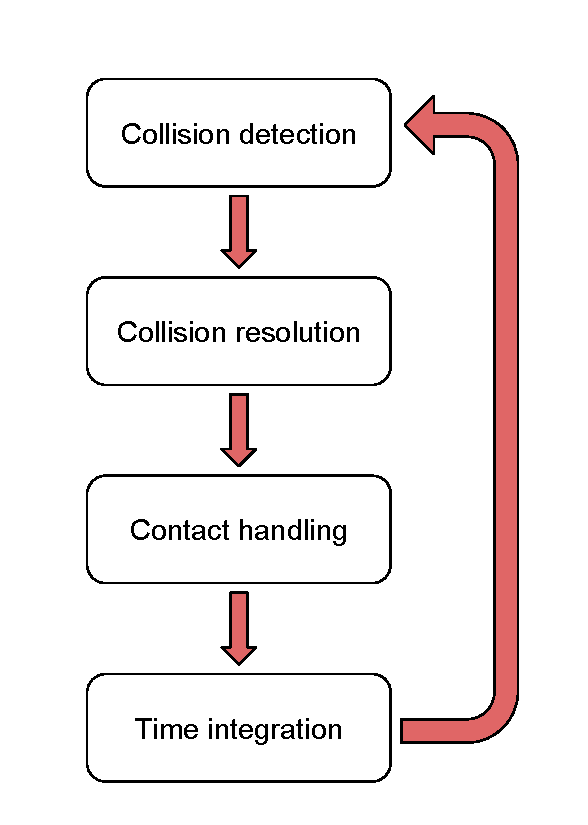
\includegraphics[width=0.5\textwidth]{figures/star_simul_loop2}
\caption[Modular phase description of the sub tasks of a rigid body simulator]{Modular phase description of the sub tasks of a rigid body simulator. The mid phase and narrow phase are grouped together because they are often combined for performance reasons}
\label{fig:phase_simul}
\end{figure}

\section{Collision detection}
\begin{figure}
\center
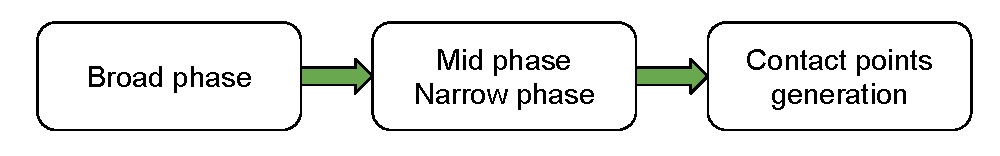
\includegraphics[width=0.9\textwidth]{figures/STAR_collision_v2}
\caption[Collision detection]{Modular description of the collision detection in a physics engine.}
\label{fig:star_collision}
\end{figure}

Collision detect is broken into three phases called the \emph{broad phase}, the \emph{mid phase} and the \emph{narrow phase}. 

During the broad phase, objects are approximated by simple geometric primitives. Distances between such geometric shapes are easy to compute. Spheres are usually used. If such spheres do not overlap, then neither do the actual objects.

When an object has a complex shape, an additional phase called the mid phase separates the object into several simpler shapes to detect collisions. Finally the narrow phase uses the exact geometries of the object to find the contact points. These are then used in the collision resolution part of the simulation loop.

We won't discuss collision detection further. For our foreseen application it is sufficient to know that simpler shapes are easier to handle. For further discussion, different possible implementations are detailed in \cite{jimenez20013d}.

\section{Collision resolution}
When bodies collide, high forces of very short duration are exerted. In the case of rigid bodies the duration is infinitesimal and the forces become infinite. This is problematic because we can see from \cref{eq:newton1} that infinite forces yield infinite accelerations which makes direct integration of that equation impossible and breaks the simulation loop.

A solution to this was proposed by Mirtich in \cite{mirtich1996impulse}. The idea is to use the standard integration rule of the simulator up to the collision, use an impulse-momentum based collision rule to determine the velocities after impact and then resume the integration.

Several collision rules exist. Newton's Hypothesis states that 
\begin{align*}
\mathbf{v}_n^+ &= e\mathbf{v}_n^-
\end{align*}
where $\mathbf{v}_n^+$ is the relative normal velocity after impact, $\mathbf{v}_n^-$ is the relative normal velocity before impact and $e \in [0, 1]$ is called the coefficient of restitution. When $e=1$ the collision is perfectly elastic and when $e=0$ all the energy is lost.

\section{Formulating the nonlinear complementarity problem (physics model)}
\subsection{Kinematics}
The position of an object in a 3D space is given by a vector $\mathbf{p} \in R^3$ from the origin of an inertial frame to the body fixed frame. The orientation of an object in a 3D space can be represented in different ways. Usually it is represented by either Euler angles or unit quaternions ($Q_s, Q_x, Q_y, Q_z$)

The translational velocity is usually noted $\mathbf{v} \in \mathcal{R}^3$. The rotational velocity $\mathbf{w} \in \mathcal{R}^3$ describes the rate at which the body rotates.

\subsection{Newton-Euler}
The Newton-Euler equations describe how forces and moments modify the velocities of an object through acceleration.

\begin{align}
m\dot{\mathbf{v}} &= \mathbf{f} \label{eq:newton1}\\
\mathbf{I}\dot{\mathbf{\omega}} + \mathbf{\omega} \times \mathbf{I}\omega &= \mathbf{\tau}
\end{align}

\subsection{Friction}
\begin{figure}[htp]
\center
\begin{subfigure}[b]{0.45\textwidth}
	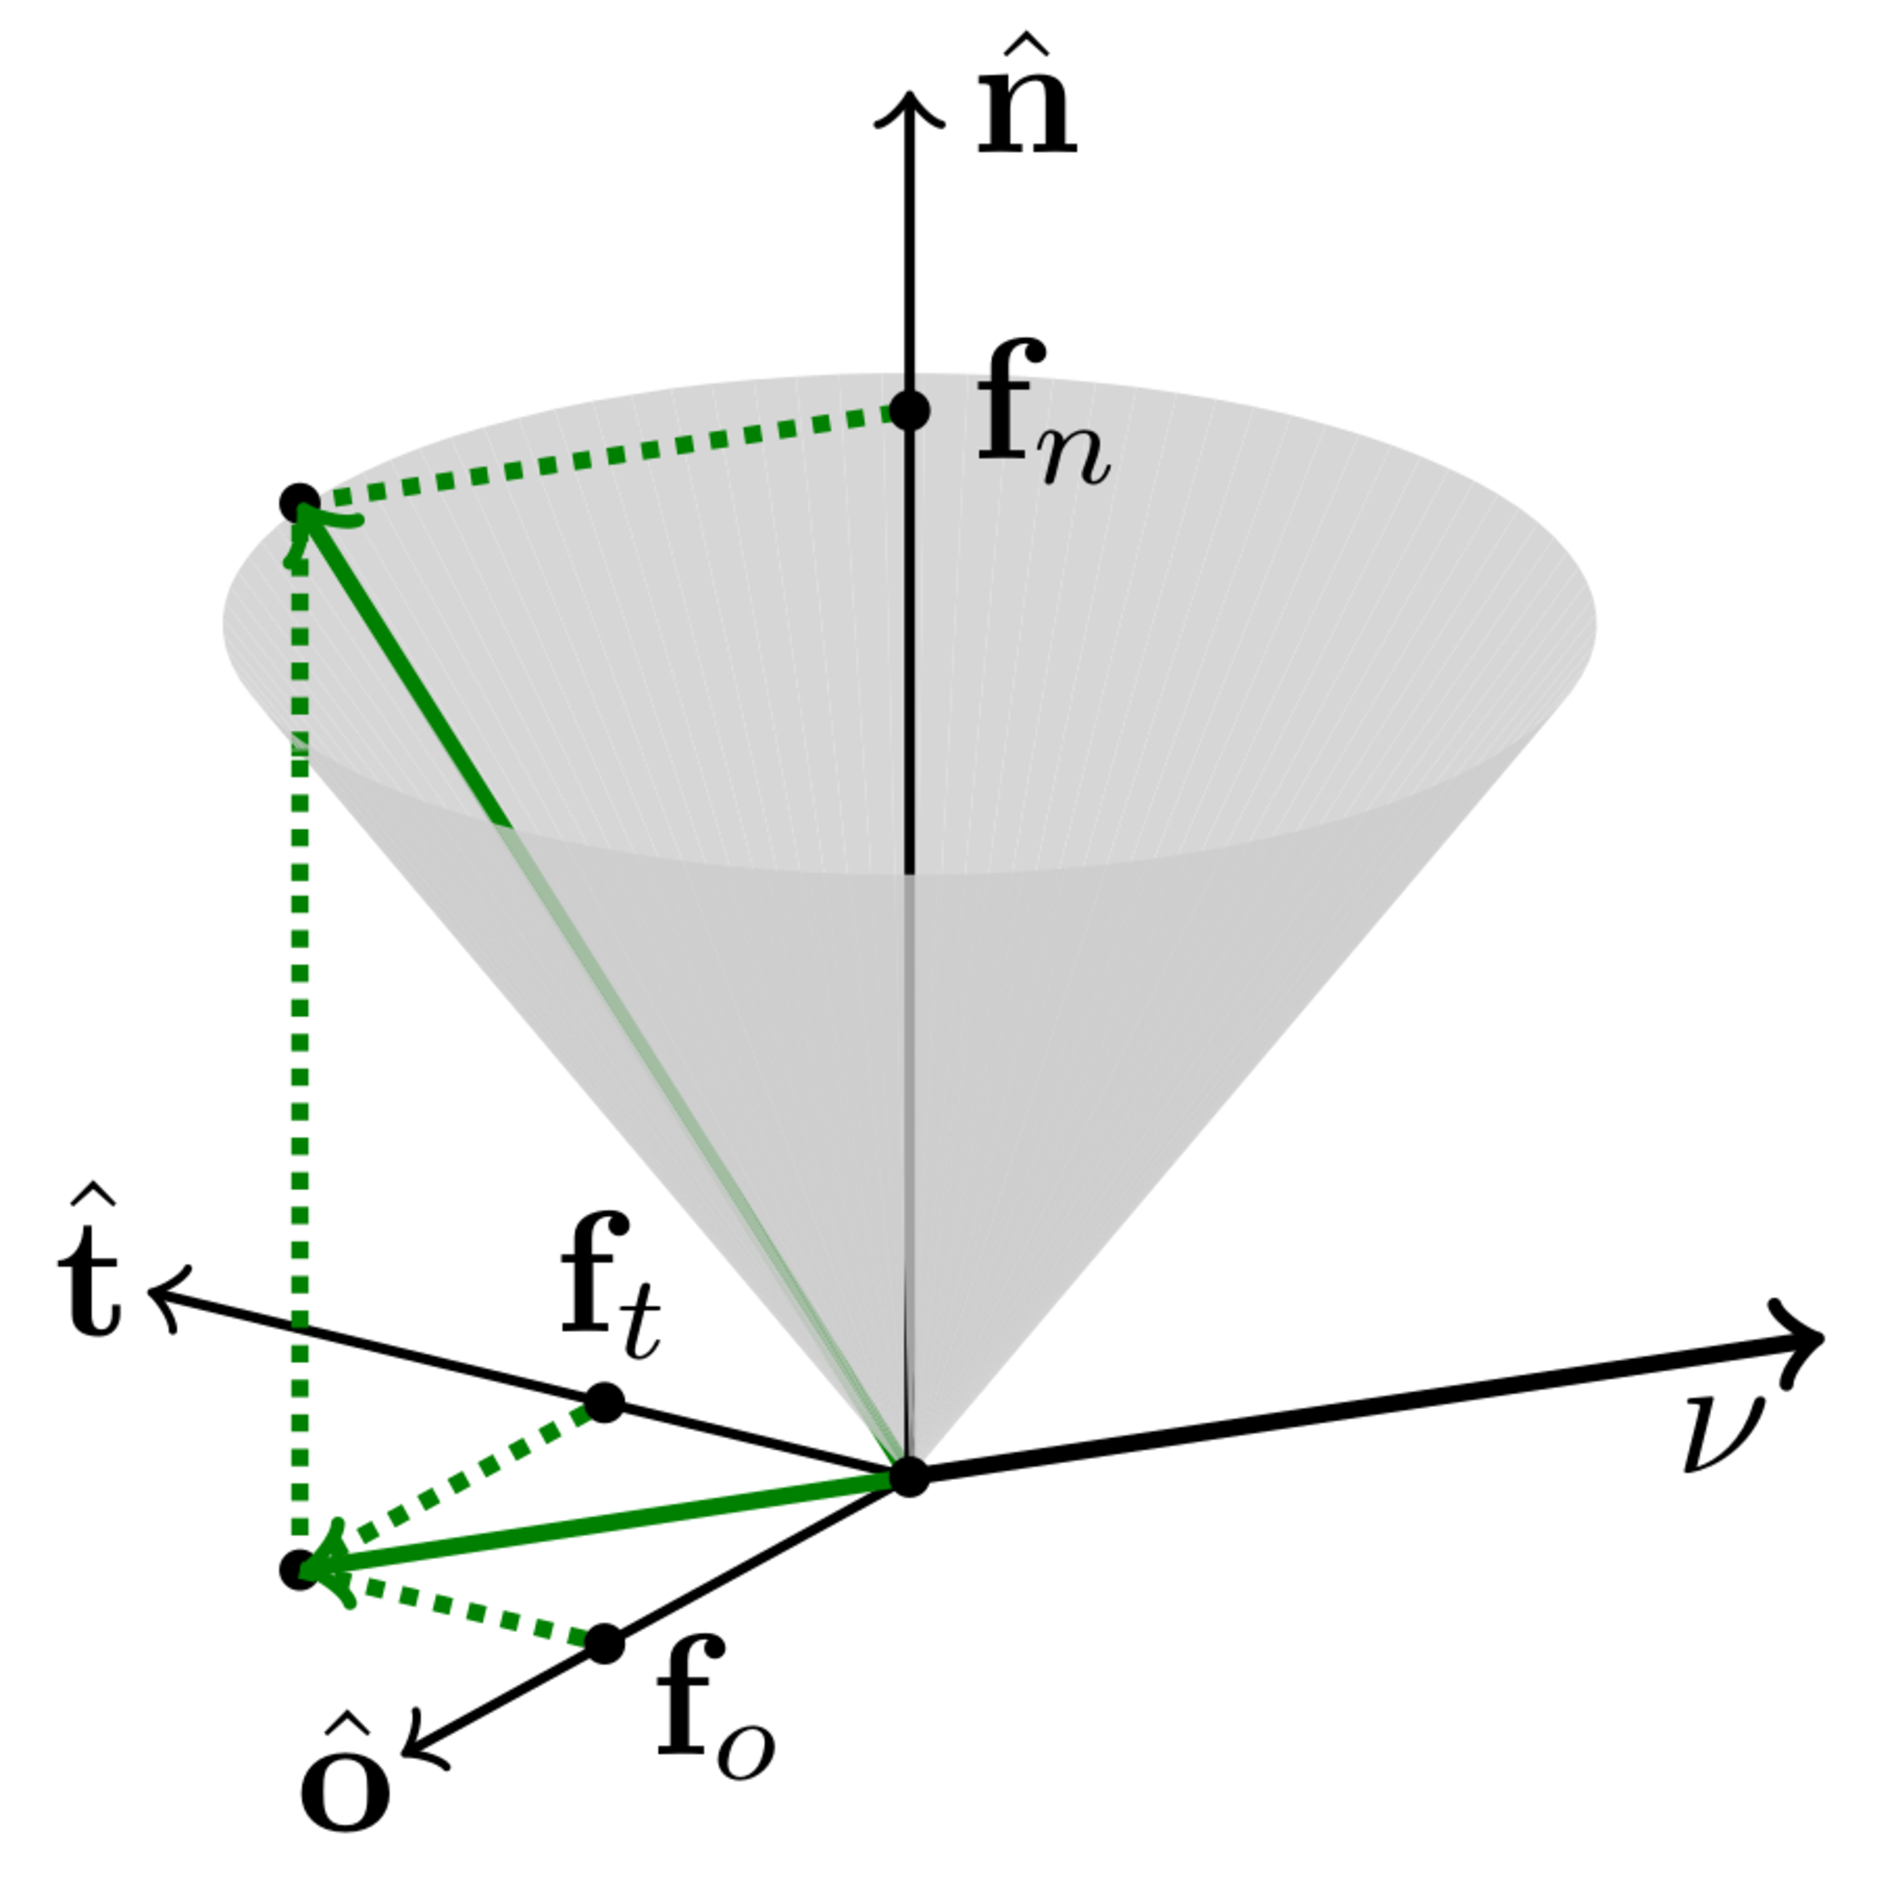
\includegraphics[width=\textwidth]{figures/friction_cone}
	\caption{A friction cone}
	\label{fig:friction_cone}
\end{subfigure}
\hfill
\begin{subfigure}[b]{0.47\textwidth}
	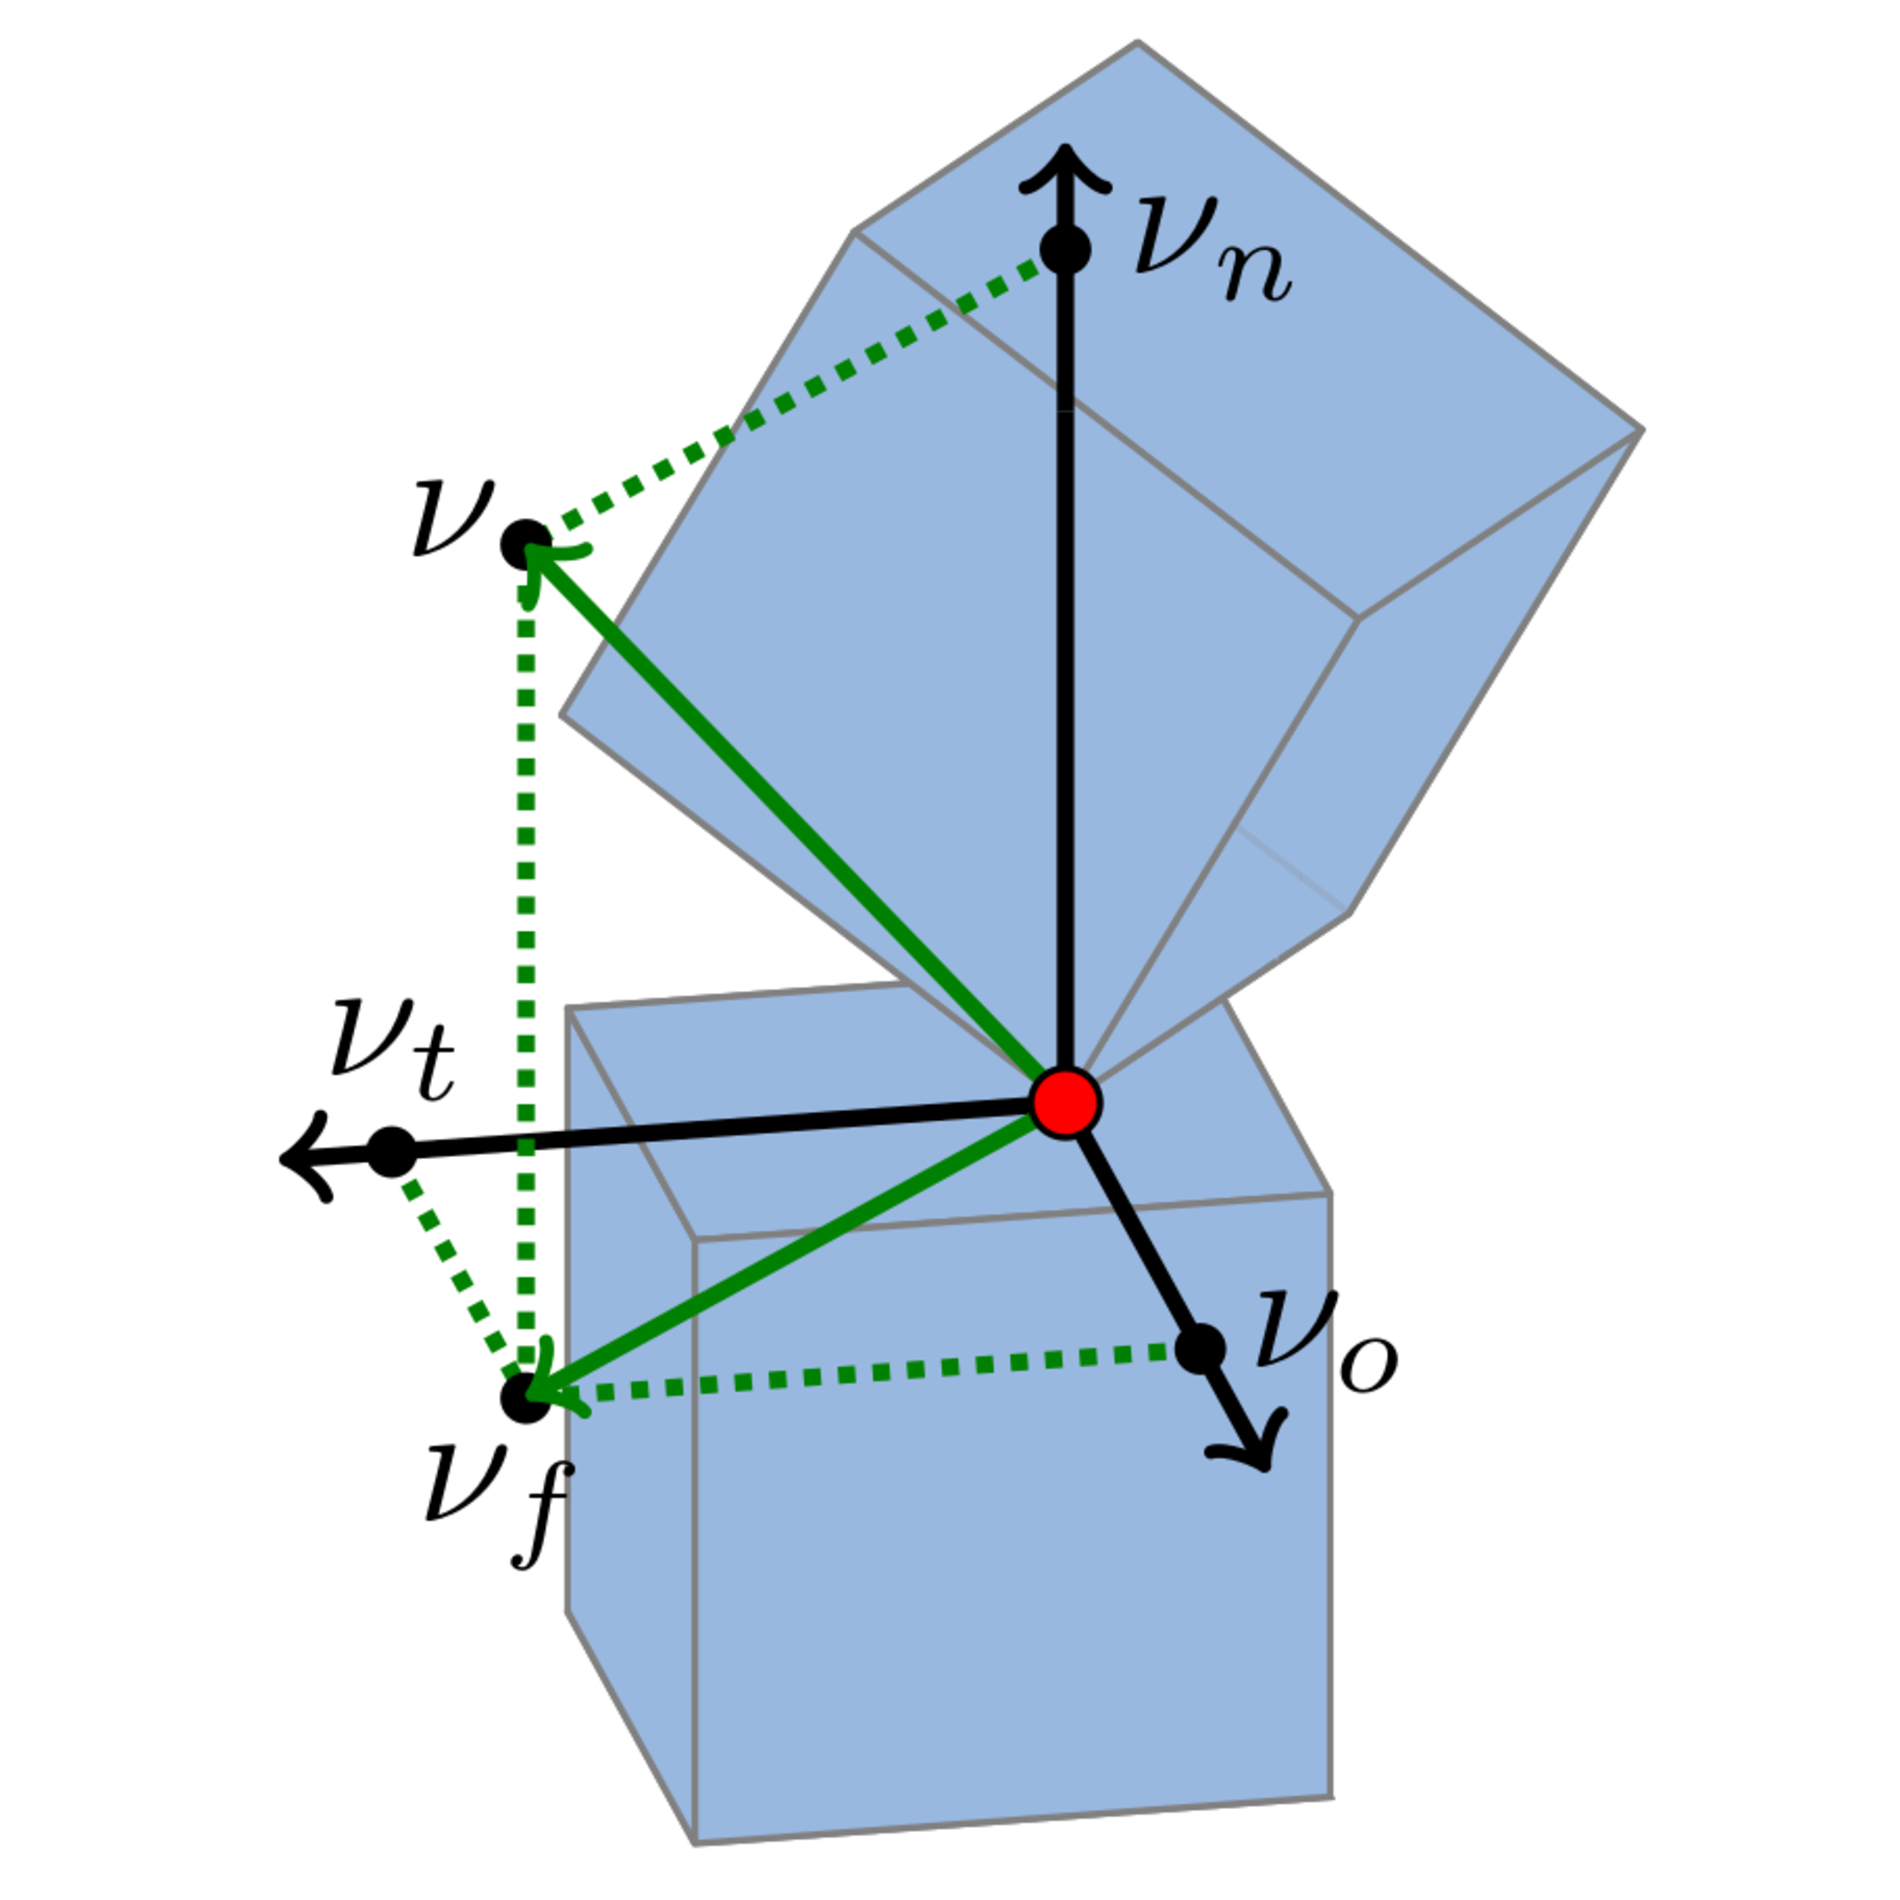
\includegraphics[width=\textwidth]{figures/friction_cube}
	\caption{Contact velocities}
	\label{fig:friction_cube}
\end{subfigure}
\caption[Friction cone and relative velocities]{Friction cone of a contact and decomposition of the contact force and relative velocity}
\label{fig:ph}
\end{figure}

Friction is the most complex type of force a physics engine must deal with. 

\subsection{Constraints}
